% !TeX root = ../../ZF_bmicha_Ana.tex
\subsection{Flächenberechnungen \texorpdfstring{\hfill S.75}{S.75}}
    \textit{Hinweis: Für die Lösunge folgender Formeln muss der Betrag genommen werden, da eine Fläche immer positiv sein muss.}
    
    \vspace{0.5em}
    \begin{itemize}
        \item Parametrisierung $\rvec=(x(t),y(t))^T$ \hfill
    \end{itemize}
    \begin{minipage}{0.65\linewidth}
        \vspace{-1em}
        \begin{itemize}
        \item[]  $\displaystyle A= \int_{t_1}^{t_2} y \dxt \, dt$
        \item[] $x(t)$ monoton
        \item[]
        \end{itemize}
    \end{minipage}
    \begin{minipage}{0.34\linewidth}
        
\includegraphics[width=0.7\linewidth]{src/Integralrechnung/param.pdf}
    \end{minipage}
    \begin{minipage}{0.65\linewidth}
        \begin{itemize}
            \item Sektorfläche
            \item[]  $\displaystyle A= \frac{1}{2} \int_{t_1}^{t_2} (x \dyt - y \dxt) \, dt$ 
            \item[] $t\mapsto (x(t),y(t))$ injektiv auf $(t_1,t_2)$ und stetig diff'bar
            \end{itemize}
            \item[]
    \end{minipage}
    \begin{minipage}{0.34\linewidth}
            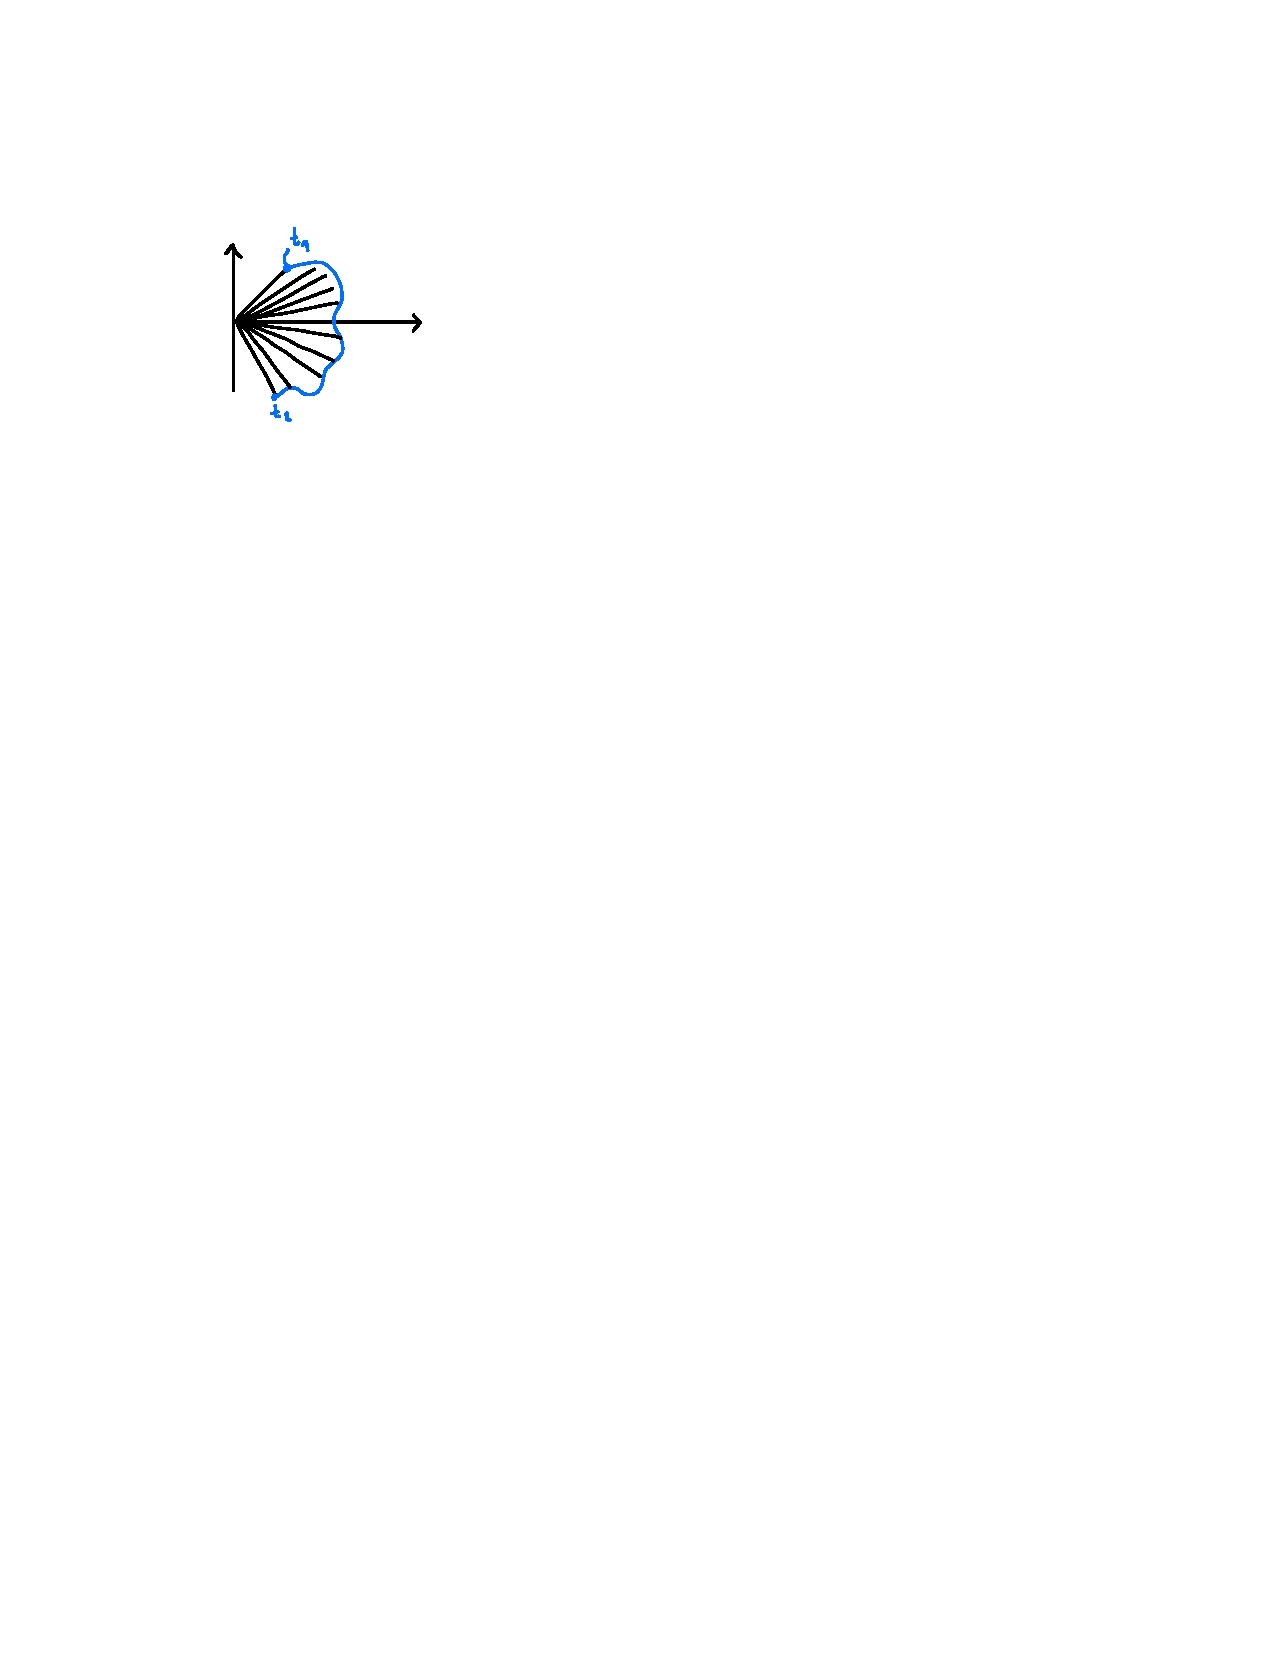
\includegraphics[width=0.6\linewidth]{src/Integralrechnung/sektor.pdf}
    \end{minipage}
    \begin{minipage}{0.65\linewidth}
        \begin{itemize}
            \item Polarkoordinaten
            \item[] $ \displaystyle A= \frac{1}{2} \int_{\varphi_1}^{\varphi_2} \rho^2(\varphi) \, d\varphi $
        \end{itemize}
    \end{minipage}
    \begin{minipage}{0.34\linewidth}
        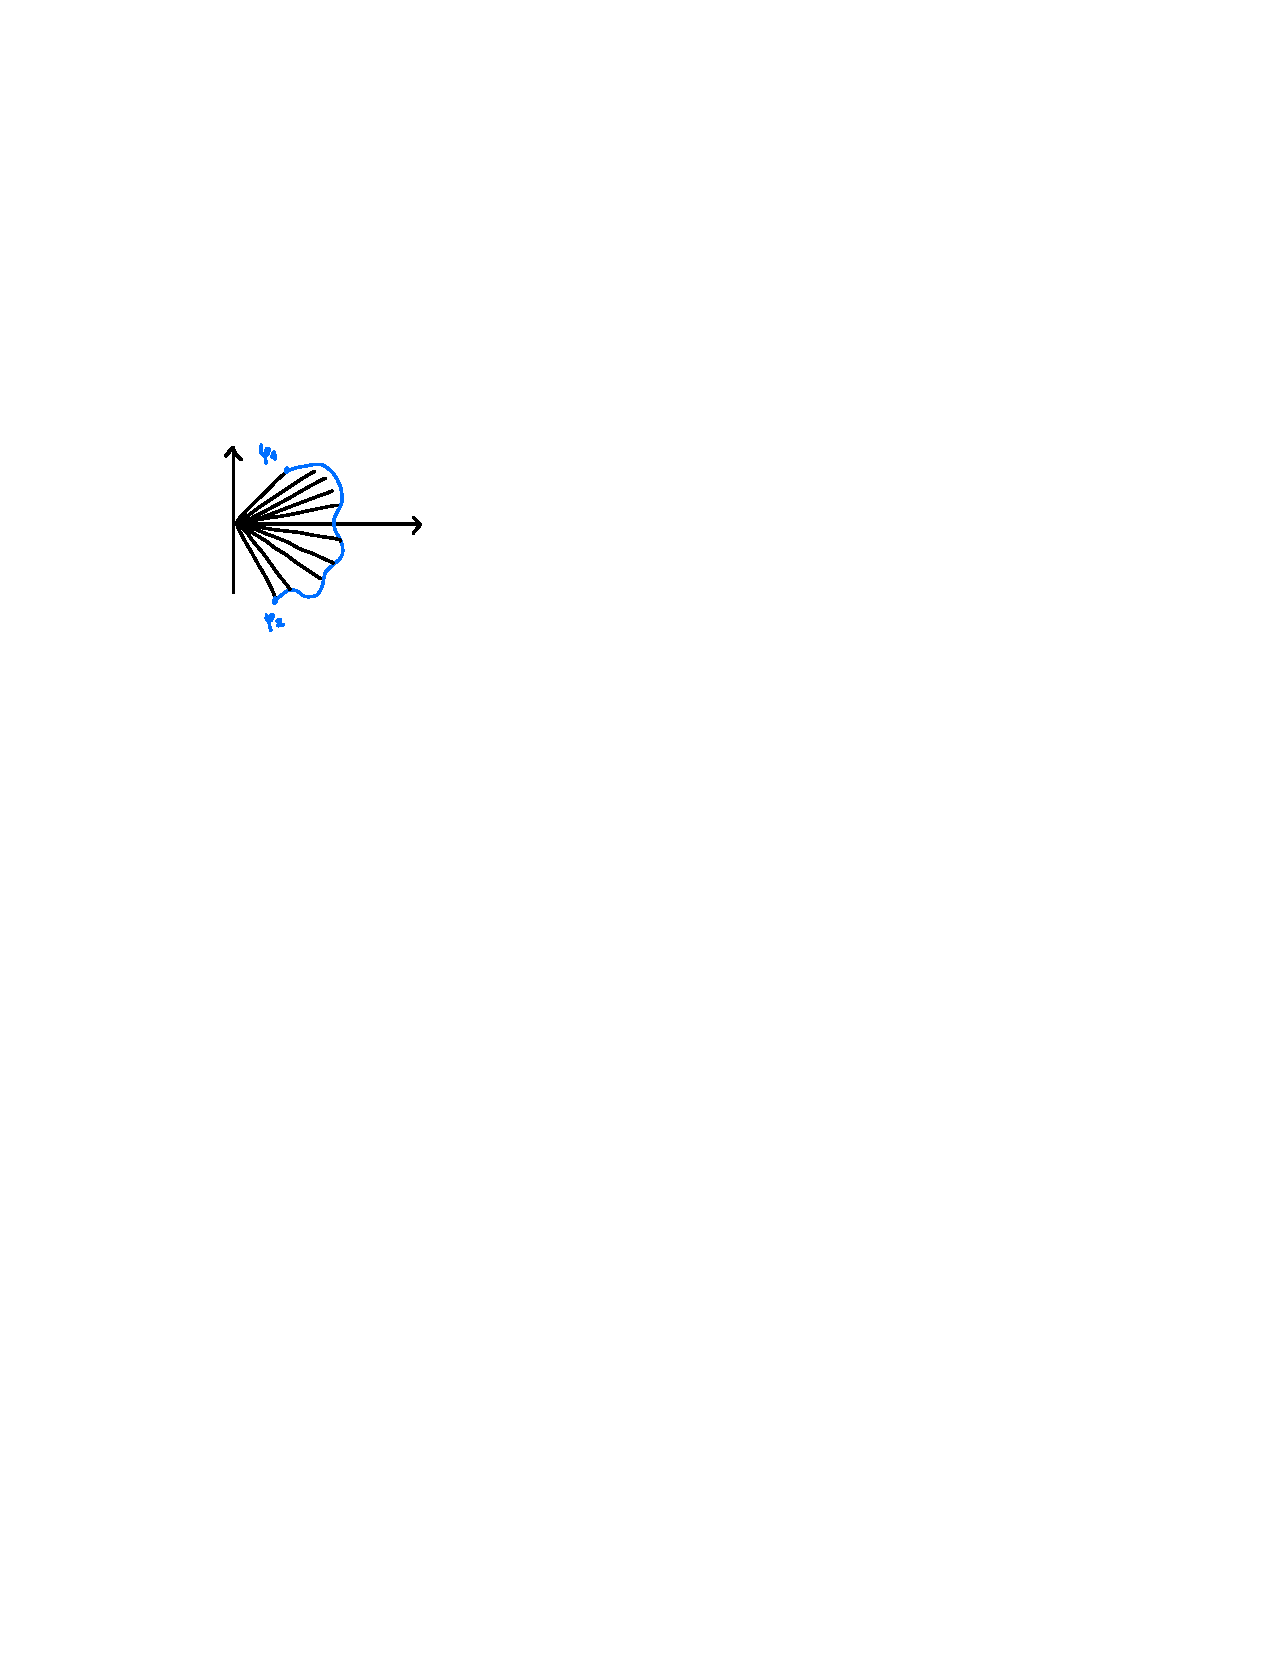
\includegraphics[width=0.6\linewidth]{src/Integralrechnung/polar.pdf}
    \end{minipage}

    
% \subsection{Flächenberechnungen}
%     \begin{minipage}{0.49\linewidth}
%         \begin{itemize}
%             \item Parametrisierung  
%             \begin{center}
%                 $\rvec=(x(t),y(t))^T$
%             \end{center}

%             $$
%             A= \int_{t_1}^{t_2} y \dxt \, dt
%             $$
%             \item Sektorfläche
%             $$
%             A= \frac{1}{2} \int_{t_1}^{t_2} (x \dyt - y \dxt) \, dt 
%             $$
%             \item Polarkoordinaten
%             $$
%             A= \frac{1}{2} \int_{\varphi_1}^{\varphi_2} \rho^2(\varphi) \, d\varphi
%             $$
%         \end{itemize}
%     \end{minipage}
%     \begin{minipage}{0.38\linewidth}
%         
\includegraphics[width=\linewidth]{src/Integralrechnung/param.pdf}
%         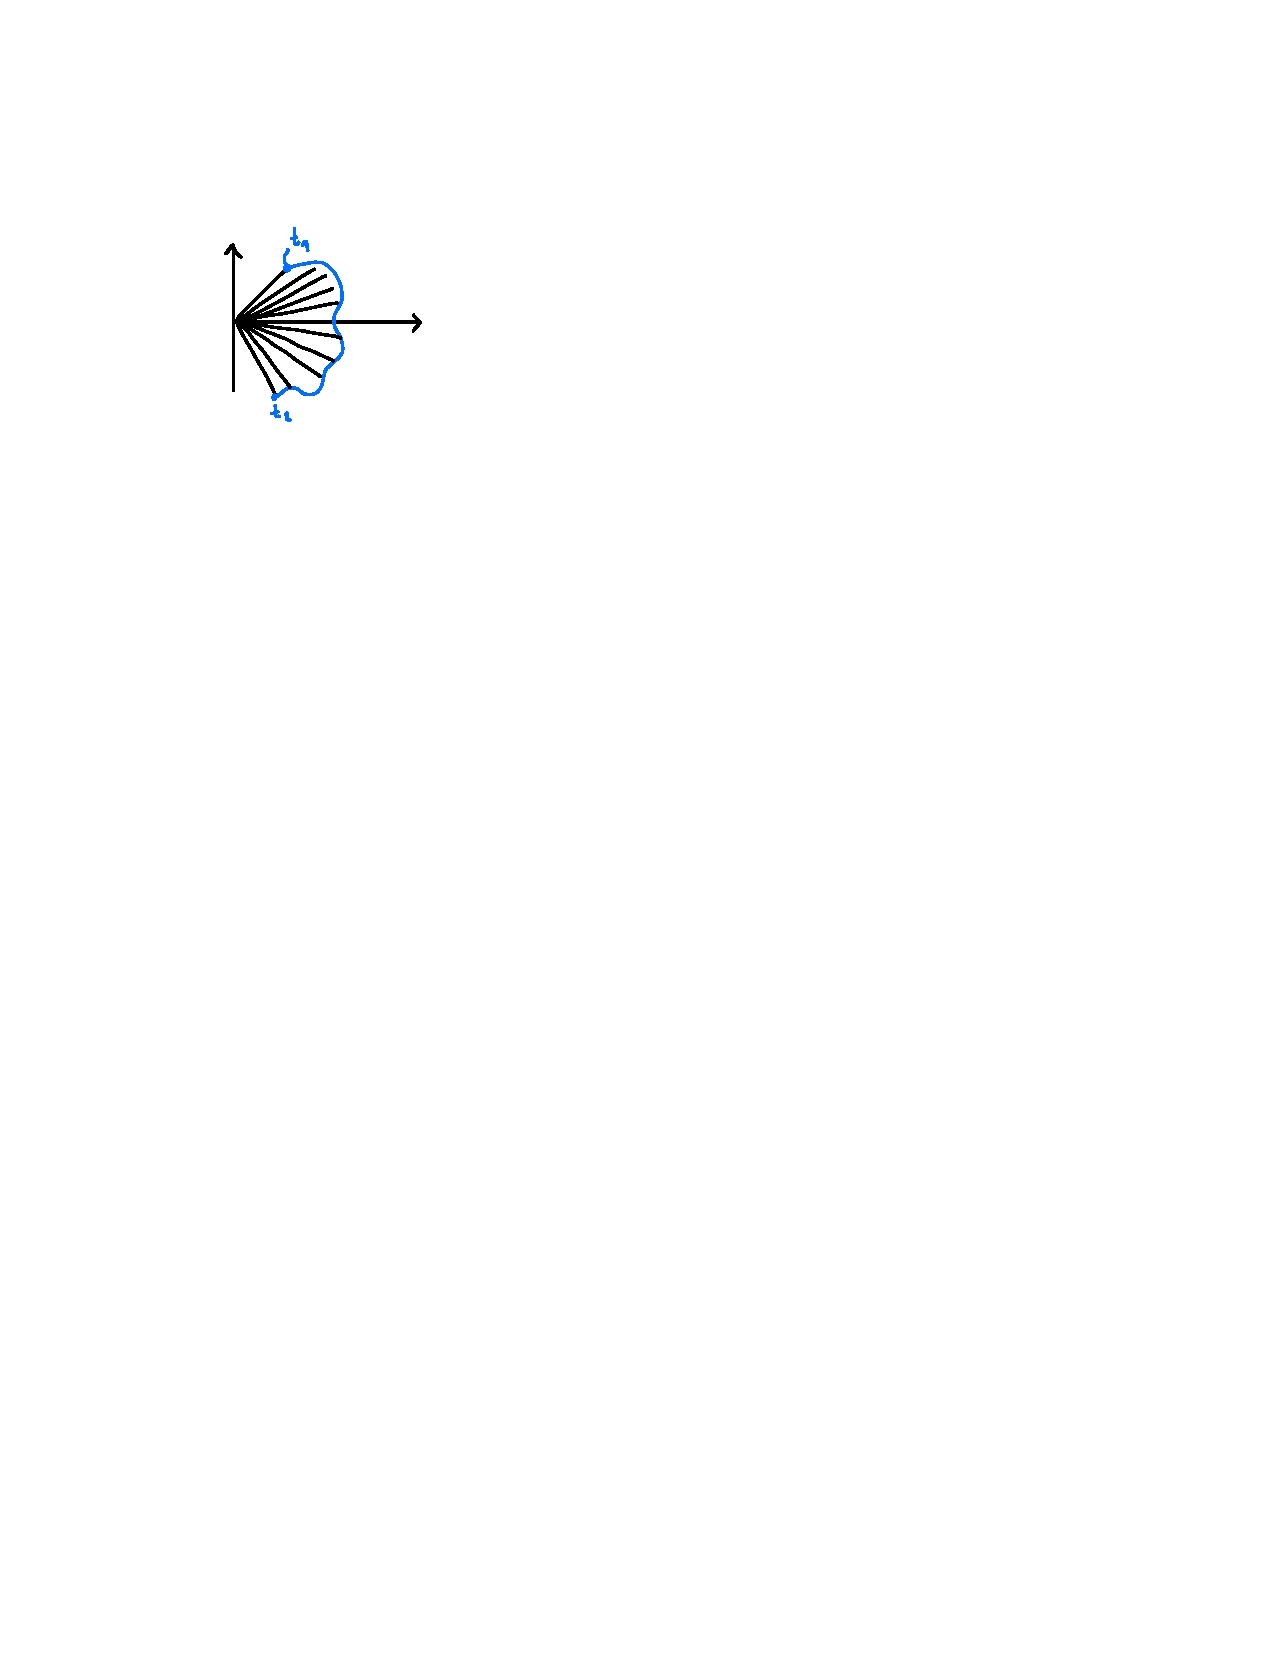
\includegraphics[width=\linewidth]{src/Integralrechnung/sektor.pdf}
%         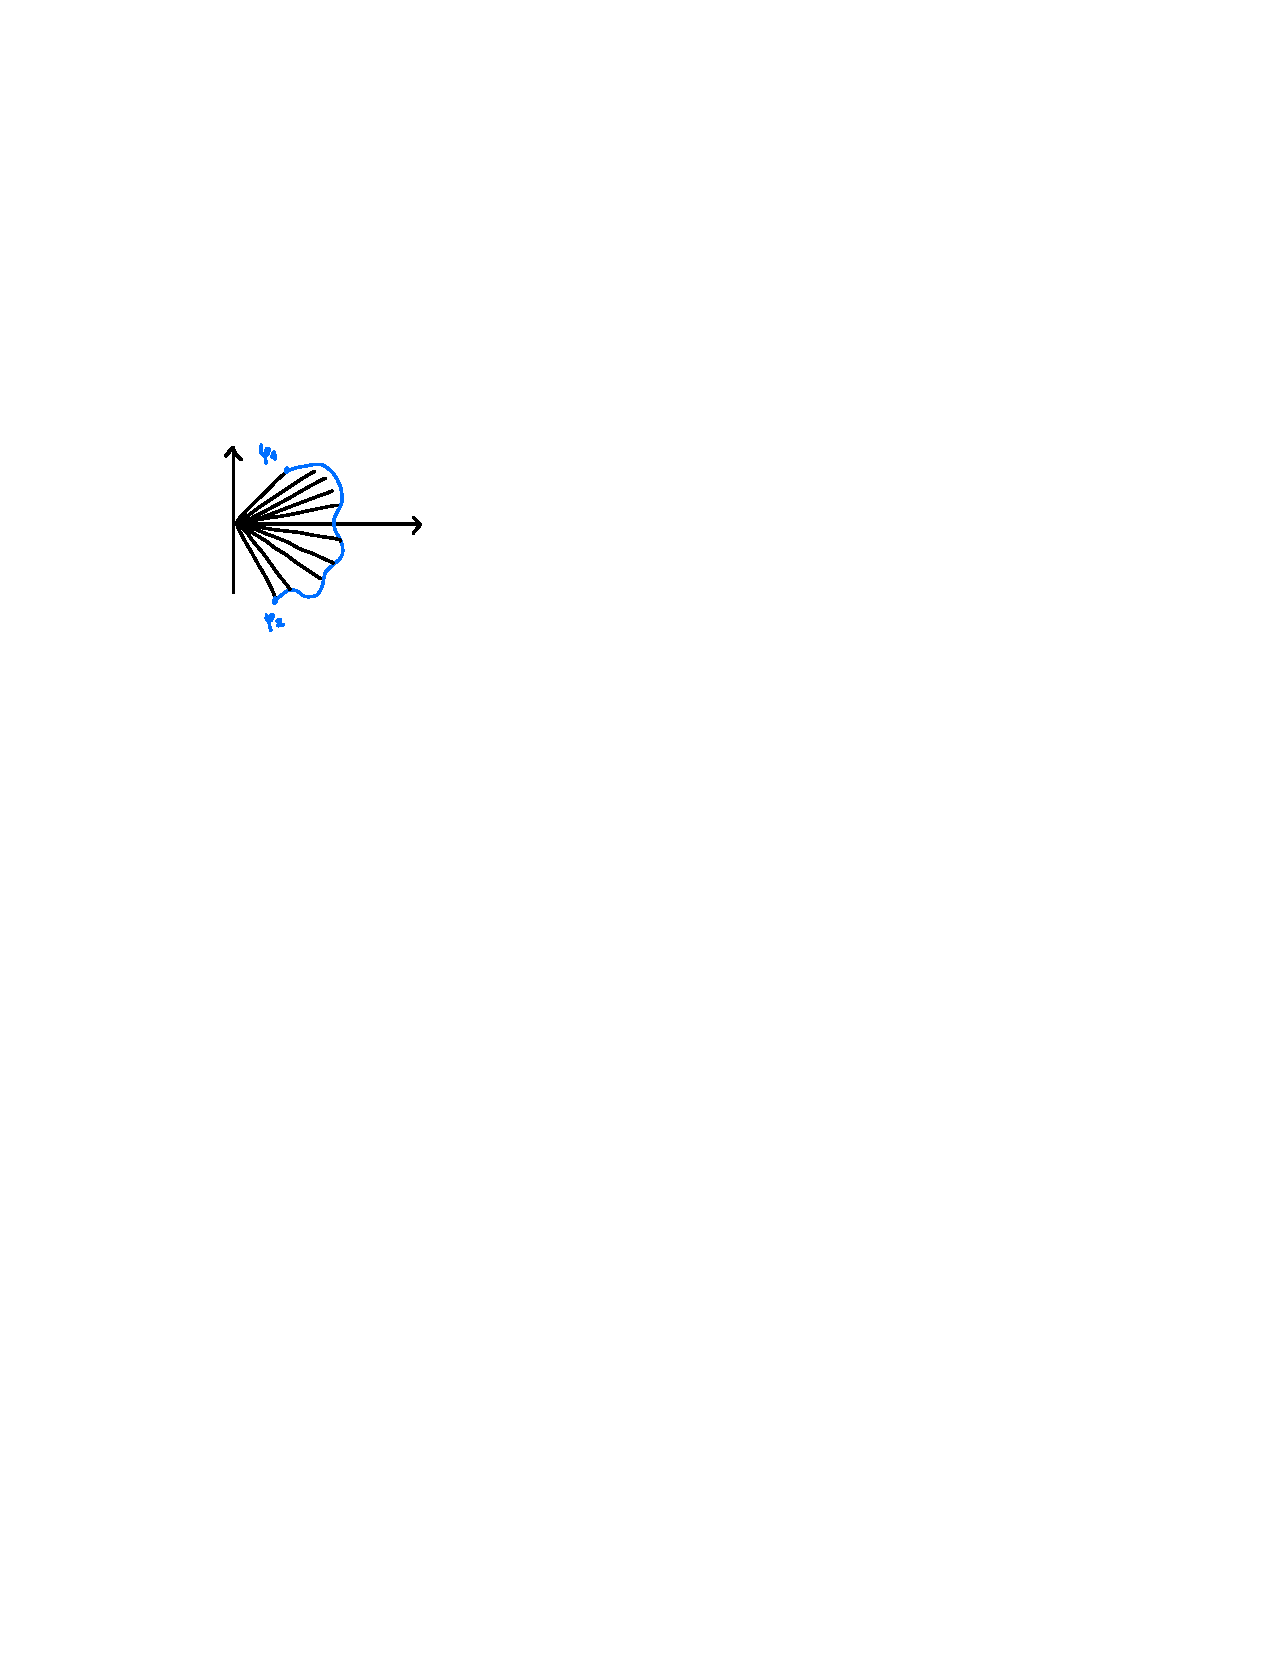
\includegraphics[width=\linewidth]{src/Integralrechnung/polar.pdf}
%     % \end{minipage}